\chapter{HowTo Document CCarat} 

\newcommand{\test}[1]{\vec{#1}}

\section{Usage}

In the \verb|/doc/technical_reports| folder, type
\begin{itemize}
\item \verb|./configure|
\item \verb|make|
\end{itemize}


\section{HowTo create a new report}

\begin{enumerate}
  \item create a new folder \verb|src_project|
  \item create a new file \verb|src_project.tex|
  \item start the file with \verb|\chapter{Project Title X|
  \item run \verb|./configure| --> your new folder should be mentioned on the screen and should appear on the screen and in the Makefile. Also, all your eps files should be mentioned in the begining of the Makefile.
\end{enumerate}


\section{Working with all the gimmiks using latex}
If you want to work without all the make magic using your editor of choice, do the following:
After creating your folder and main file and running configure, do
\begin{enumerate}
 \item copy the file \verb|temp/single_report_project.tex| to your \verb|src/src_project| folder
 \item delete \verb|inputpath| and \verb|figurepath| stuff from this file
 \item use \verb|latex single_report_project| as usual
\end{enumerate}
This ensures that you have all the packages and conform to the standard of the configure script and, therefore, the general CCARAT (oops, he said it again...) documentation.


\section{Technic}

The reports are produced with PDF\LaTeX.

\subsection{Basics}

You can include files as
\begin{verbatim}
Lorem ipsum dolor sit amet, consectetuer adipiscing elit. Proin interdum aliquam urna. Donec lorem. Phasellus nisl. Nam gravida mauris a elit. Vestibulum mattis dolor ac enim. Nunc eget libero vitae lectus faucibus placerat. In risus. Cras purus. Vivamus placerat, augue ut auctor tempus, mi mi tincidunt ipsum, quis consequat urna nulla at ante. Suspendisse posuere, erat sit amet malesuada blandit, lorem mi egestas justo, nec tempus diam quam quis mi. Proin nec elit. Praesent cursus. Curabitur aliquet, odio in euismod suscipit, mi sem hendrerit turpis, eget varius lorem lectus eget arcu. Vestibulum vel nibh. Nam euismod feugiat nulla. Nullam nisi libero, mattis ut, mattis cursus, interdum sed, diam.

Proin non massa id risus vehicula dapibus. Integer odio elit, pretium ut, dictum et, bibendum ac, mi. Sed et nisl. Sed vulputate porttitor est. Pellentesque diam. Sed turpis. Aliquam pulvinar tincidunt sem. Nulla risus ligula, consequat sit amet, sagittis non, sagittis eu, massa. Integer nunc. Pellentesque habitant morbi tristique senectus et netus et malesuada fames ac turpis egestas. Suspendisse pharetra hendrerit lorem. Proin pede. Pellentesque sed nulla.

Cras congue. Vestibulum nulla tortor, malesuada a, pulvinar at, suscipit et, nunc. In at lacus et libero porttitor ullamcorper. Donec turpis. Quisque rutrum accumsan magna. In hac habitasse platea dictumst. Duis eget nisi. Aliquam scelerisque lacus in nulla laoreet commodo. Nulla facilisi. Integer sodales condimentum arcu. Vestibulum quam. Sed gravida pellentesque eros. Pellentesque nec tortor. Aenean tincidunt, metus ac interdum ullamcorper, lacus odio pellentesque diam, vitae pretium purus mi sed velit.

Duis tristique rutrum risus. Etiam malesuada elementum eros. In mauris. Vestibulum tempus, arcu at molestie congue, lacus mi dignissim pede, in posuere mauris arcu sit amet justo. Nullam eu orci sit amet ipsum fringilla dictum. Vestibulum semper ipsum vitae pede. Etiam mi. Ut sed libero. Ut vitae magna at mauris dapibus rutrum. Mauris a risus. Maecenas aliquam elit eu felis blandit varius. Quisque vitae felis. Vestibulum eget orci in orci commodo lobortis. Ut augue felis, adipiscing in, dignissim ut, ullamcorper et, est. Etiam in massa ac dolor semper consequat. Nam diam odio, venenatis non, placerat ut, sodales eget, urna. In ligula quam, ornare quis, congue ut, vulputate non, eros. Phasellus pretium.

Maecenas sed augue. Vestibulum id felis et quam consectetuer imperdiet. Suspendisse vitae elit a ligula consequat pharetra. Curabitur vel est quis nunc mollis ultrices. Praesent sollicitudin purus at sapien. Sed justo velit, elementum vitae, vehicula eu, ornare sed, diam. Nam ligula. Sed laoreet erat vitae nulla. Phasellus iaculis nibh. Phasellus porttitor. Curabitur hendrerit suscipit pede. Sed tincidunt, purus placerat nonummy lobortis, ante augue semper dolor, at elementum mauris elit ut nisl. Etiam facilisis libero bibendum nisl. Donec dapibus consectetuer lacus.

Proin augue. Mauris at libero in diam aliquet blandit. Nullam mauris mauris, vestibulum at, suscipit sed, euismod pretium, nisl. Sed sollicitudin nulla id velit. Aliquam vel turpis. Vivamus arcu tortor, tristique at, lacinia eget, ultricies in, turpis. Vivamus urna sem, posuere eu, rhoncus in, imperdiet eu, tortor. Maecenas malesuada arcu non mauris. Sed quis tellus. Nunc ultricies. Etiam ornare placerat magna. Curabitur rutrum erat quis orci tincidunt blandit. Sed leo. Vivamus rutrum dapibus nisi. Nulla facilisi. 

\end{verbatim}

You can define your own commands, which won't be visible outside of your chapter
\newcommand{\testbastel}[1]{\vec{#1}}
\begin{verbatim}
\newcommand{\testbastel}[1]{\vec{#1}}
\end{verbatim}
Keep all your newcommands inside your own files to avoid cluttering of the templates. The templates are only allowed to be changed to add packages via \verb|\usepackage{}|.

% Use \verb|\input| instead of \verb|\include|. The additional \verb|.aux| file confuses \LaTeX and always requires additional recompiling, whether crossreferences are correct or not.

\subsection{Figures}

All figures have to be provided in EPS format. This allows usage of latex and pdflatex. All paths to pictures have to be in relative paths with respect to the \verb|src_example.tex| file.

Do not use endings in you including statement.
\subsubsection{Binary Images}
\begin{verbatim}
\begin{figure}
\begin{center}
  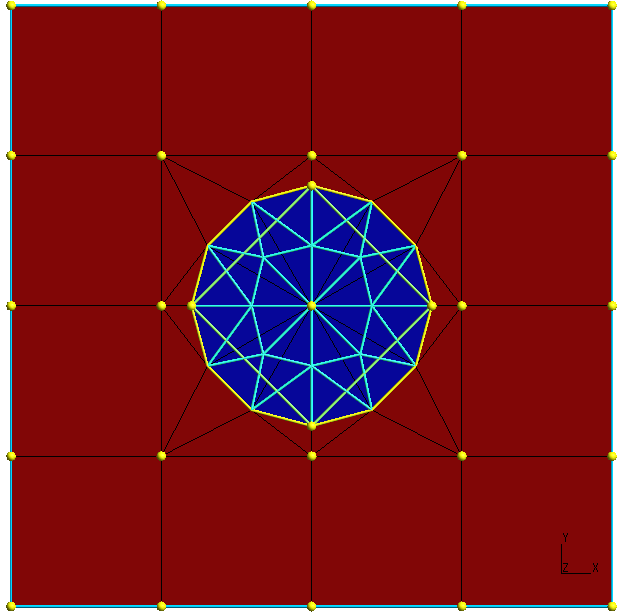
\includegraphics[width=0.5\textwidth]{figures/new_interface_mesh_show_all_meshes}
  \caption{Included PNG file}
\end{center}
\end{figure}
\end{verbatim}

\subsubsection{EPS Images}
\begin{verbatim}
\begin{figure}
\begin{center}
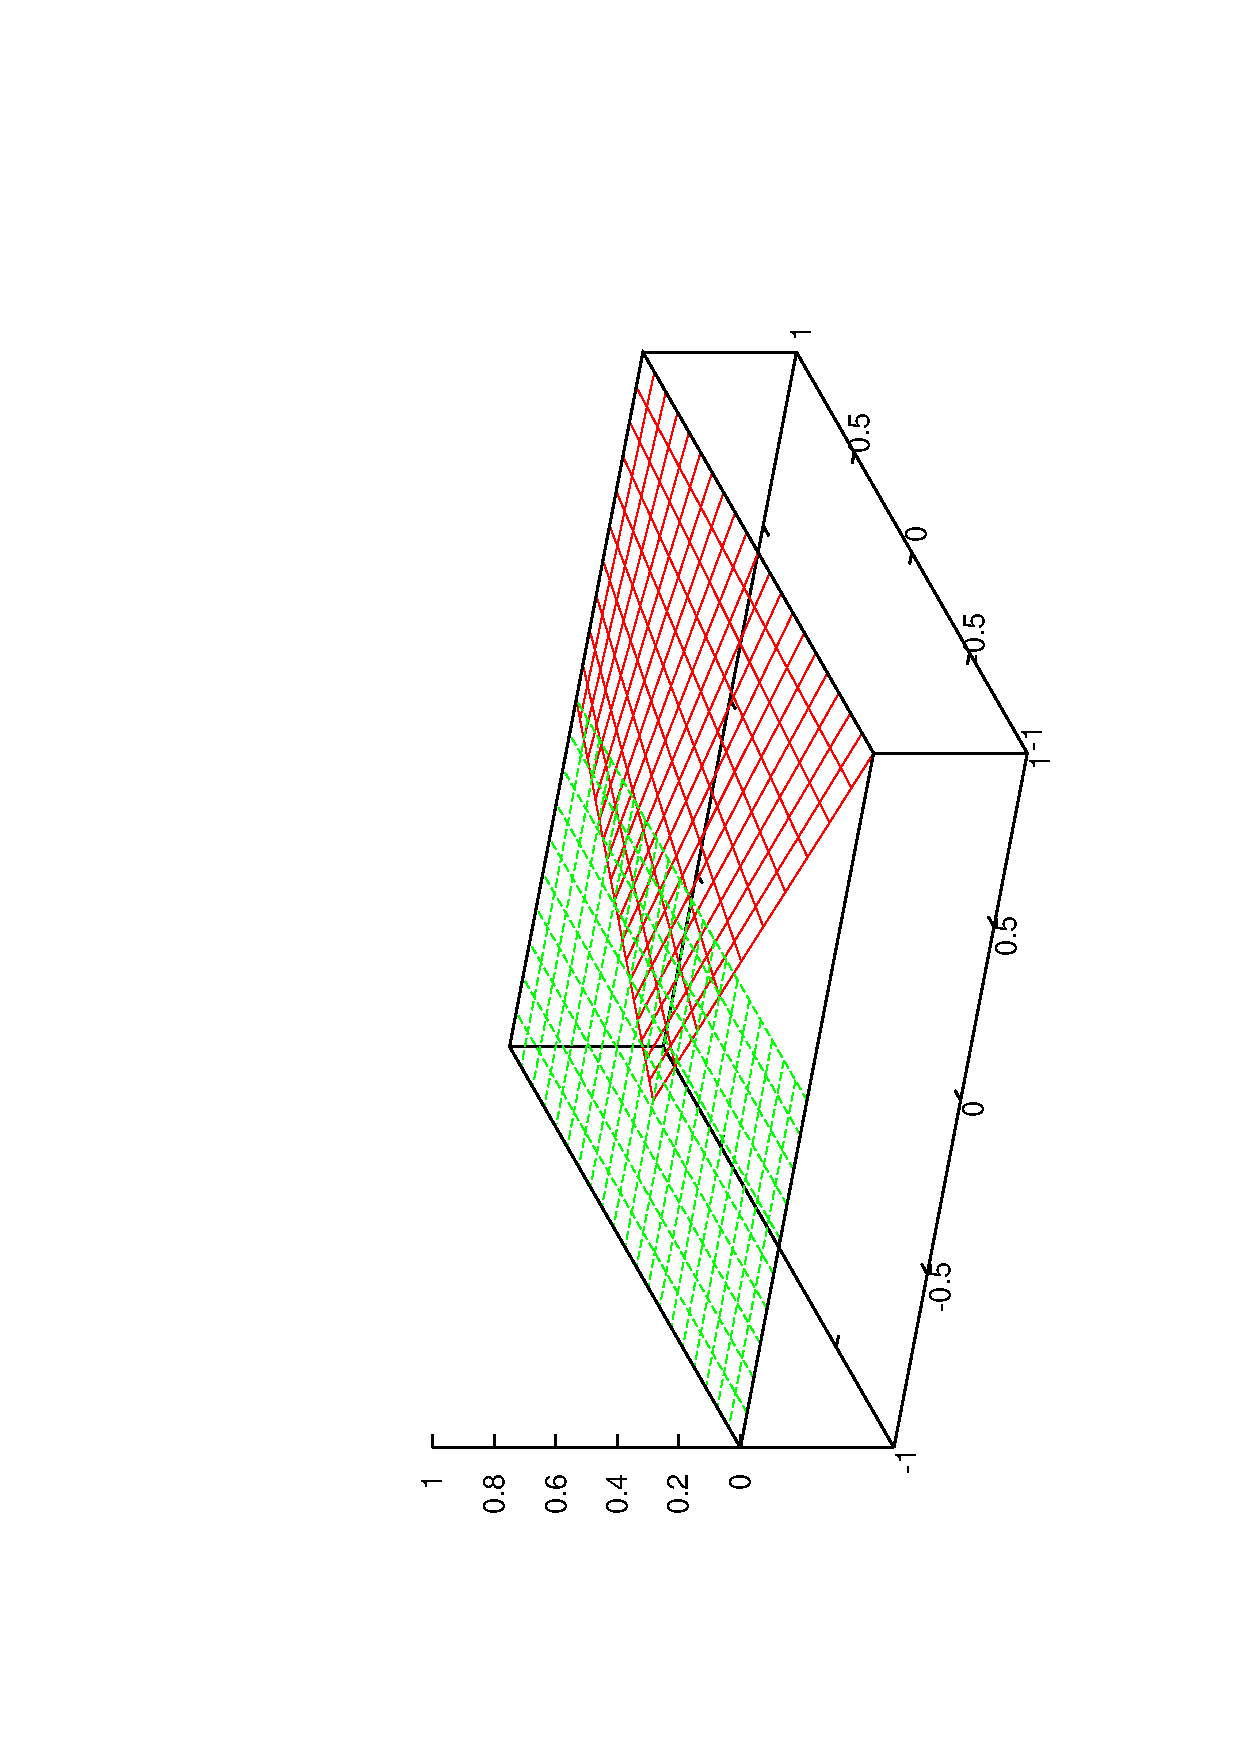
\includegraphics[angle=-90,width=0.5\textwidth]{figures/xfem_N1}
  \caption{Included EPS/PDF file, depending whether \LaTeX or PDF-\LaTeX was used}
\end{center}
\end{figure}
\end{verbatim}

eps images will be translated automatically via \verb|epstopdf| to a little pdf file of the same size (bounding box) and is always uptodate with the eps file during compilation of the documents.
